\documentclass[letterpaper, 11pt]{article}
\usepackage[utf8]{inputenc}
\usepackage[letterpaper, portrait, margin=1in]{geometry}
\usepackage{pgfplots}
\pgfplotsset{width=10cm,compat=1.9}
\usepackage{hyperref}
\usepackage{textcomp}
\usepackage{siunitx}
\usepackage{amsmath}
\usepackage{cancel}
\usepackage{tikz}
\usepackage{everysel}
\usepackage{ragged2e}
\usepackage{mathdots}
\usepackage{yhmath}
\usepackage{color}
\usepackage{array}
\usepackage{multirow}
\usepackage{amssymb}
\usepackage{gensymb}
\usepackage{tabularx}
\usepackage{booktabs}
\usepackage{listings}
\usepackage{xcolor}
\usetikzlibrary{fadings}
\usetikzlibrary{patterns}
\usetikzlibrary{shadows.blur}
\hypersetup{
    colorlinks=true,
    linkcolor=black,
    filecolor=black,      
    urlcolor=blue,
}

\definecolor{codegreen}{rgb}{0,0.6,0}
\definecolor{codegray}{rgb}{0.5,0.5,0.5}
\definecolor{codepurple}{rgb}{0.58,0,0.82}
\definecolor{backcolour}{rgb}{0.95,0.95,0.92}

\lstdefinestyle{mystyle}{
    backgroundcolor=\color{backcolour},   
    commentstyle=\color{codegreen},
    keywordstyle=\color{magenta},
    numberstyle=\tiny\color{codegray},
    stringstyle=\color{codepurple},
    basicstyle=\ttfamily\footnotesize,
    breakatwhitespace=false,         
    breaklines=true,                 
    captionpos=b,                    
    keepspaces=true,                 
    numbers=left,                    
    numbersep=5pt,                  
    showspaces=false,                
    showstringspaces=false,
    showtabs=false,                  
    tabsize=2
}

\lstset{style=mystyle}

\title{COMSC-200 \\ Lab 2}
\author{Ryan Jacoby}
\date{6 September 2020}
\begin{document}

\maketitle

\section{Date}

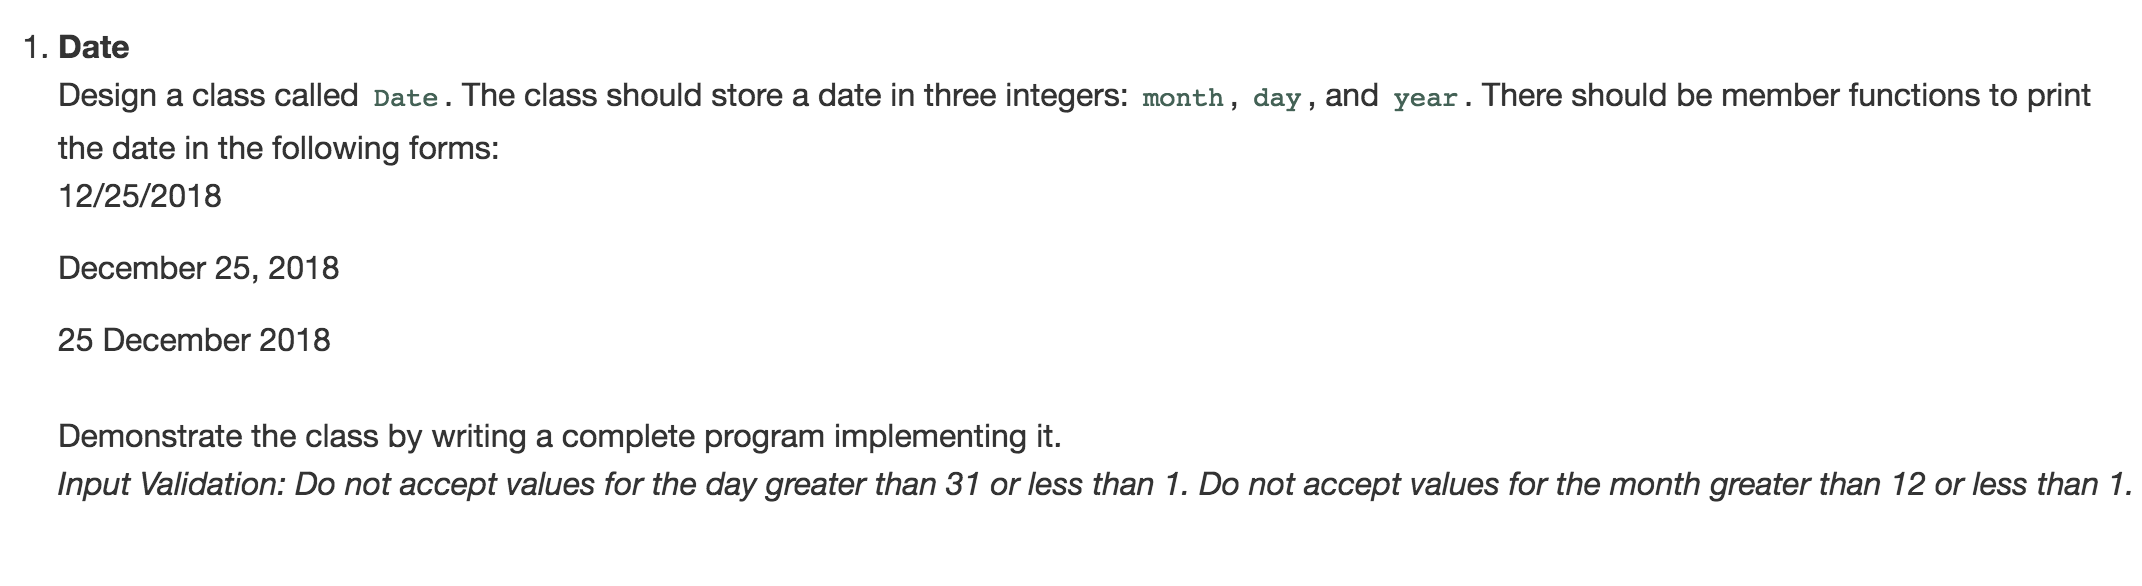
\includegraphics[scale=0.35]{date.png} 

\begin{lstlisting}[language=C++, caption=main.cpp]
// Ryan Jacoby

#include<iostream>

#include"Date.h"

using namespace std;

int main() {
    Date d = Date();
    d.setDay(6);
    d.setMonth(9);
    d.setYear(2020);

    Date d1 = Date(25, 12, 2021);

    cout << "Date 1:\n";
    cout << d.getDateA() << '\n';
    cout << d.getDateB() << '\n';
    cout << d.getDateC() << '\n';

    cout << "\nDate 2:\n";
    cout << d1.getDateA() << '\n';
    cout << d1.getDateB() << '\n';
    cout << d1.getDateC() << '\n';

    return 0;
}
\end{lstlisting}

\begin{lstlisting}[language=C++, caption=Date.h]
// Ryan Jacoby

#ifndef Date_h
#define Date_h

using namespace std;

class Date {
private:
    int day;
    int month;
    int year;
public:
    Date();
    Date(int day, int month, int year);

    void setDay(int day);
    void setMonth(int month);
    void setYear(int year);

    string getDateA();
    string getDateB();
    string getDateC();
};

#endif
\end{lstlisting}

\begin{lstlisting}[language=C++, caption=CoinImp.cpp]
// Ryan Jacoby

#include<string>

#include"Date.h"

using namespace std;

string months[] = {"January", "February", "March", "April", "May", "June", "July", "August", "September", "October", "November", "December"};

Date::Date() {
    this->day = 1;
    this->month = 1;
    this->year = 0;
}

Date::Date(int day, int month, int year) {
    if(day > 0 && day < 32) this->day = day;
    else this->day = 1;

    if(month > 0 && month < 13) this->month = month;
    else this->month = 1;

    this->year = year;
}

void Date::setDay(int day) {
    if(day > 0 && day < 32) this->day = day;
    else this->day = 1;
}

void Date::setMonth(int month) {
    if(month > 0 && month < 13) this->month = month;
    else this->month = 1;
}

void Date::setYear(int year) {
    this->year = year;
}

string Date::getDateA() {
    return to_string(this->month) + "/" + to_string(this->day) + "/" + to_string(this->year);
}

string Date::getDateB() {
    return months[this->month - 1] + " " + to_string(this->day) + "," + to_string(this->year);
}

string Date::getDateC() {
    return to_string(this->day) + " " + months[this->month - 1] + " " + to_string(this->year);
}
\end{lstlisting}

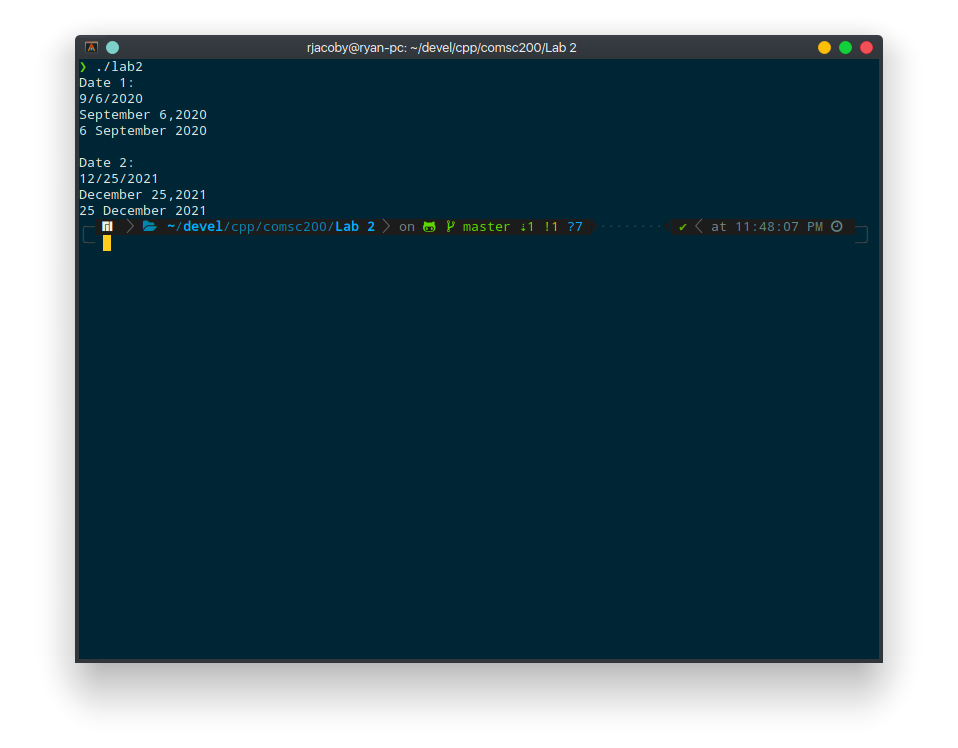
\includegraphics[scale=0.5]{date_run.png} 

\end{document}
